% =============================================================================
% COPYRIGHT AND DISCLAIMER
% =============================================================================
% This file is provided as a convenience template for competition participants.
% By using it, you accept full responsibility for compliance with all applicable
% copyright, licensing, and usage rules of the Association for Computing
% Machinery (ACM) and of any LaTeX packages you load (including, without
% limitation, the "acmart" document class and related ACM materials).
%
% Consult ACM's official publication, template, and copyright policies before
% using this setup for any purpose other than this competition. Do not assume
% that this template may be reused, redistributed, or submitted elsewhere
% without independently verifying ACM's current rules.
%
% Use of the "acmart" class, the "sigconf" option, or ACM-style formatting in
% this template does NOT mean that this report, this competition, its organizers,
% or any resulting PDF is sponsored, endorsed, affiliated with, or published by
% ACM. ACM trademarks and branding remain the property of ACM.
%
% Template packages live in preamble.tex.
% Citations live in main.bib. Edit this file with your paper content.
% =============================================================================

\documentclass[sigconf]{acmart}
% =============================================================================
% Template setup — participants normally do not edit this file.
% Author content belongs in main.tex; citations belong in main.bib.
% \documentclass lives in main.tex so Overleaf does not treat this file as root.
% =============================================================================

% --- Competition / non-ACM-submission friendly rights metadata -------------
\setcopyright{none}
\settopmatter{printacmref=false}
\acmConference[Kaggle Competition]{Filament Segmentation Challenge}{2026}{\href{https://www.kaggle.com/competitions/filament-segmentation-2026}{kaggle.com/competitions/filament-segmentation-2026}}
\acmBooktitle{Competition Report}
\acmDOI{}
\acmISBN{}

% --- Author guidance text --------------------------------------------------
% \guide{...} is gray italic while \guideStyletrue; omitted from the PDF if false.
% Flip the switch in main.tex after % =============================================================================
% Template setup — participants normally do not edit this file.
% Author content belongs in main.tex; citations belong in main.bib.
% \documentclass lives in main.tex so Overleaf does not treat this file as root.
% =============================================================================

% --- Competition / non-ACM-submission friendly rights metadata -------------
\setcopyright{none}
\settopmatter{printacmref=false}
\acmConference[Kaggle Competition]{Filament Segmentation Challenge}{2026}{\href{https://www.kaggle.com/competitions/filament-segmentation-2026}{kaggle.com/competitions/filament-segmentation-2026}}
\acmBooktitle{Competition Report}
\acmDOI{}
\acmISBN{}

% --- Author guidance text --------------------------------------------------
% \guide{...} is gray italic while \guideStyletrue; omitted from the PDF if false.
% Flip the switch in main.tex after % =============================================================================
% Template setup — participants normally do not edit this file.
% Author content belongs in main.tex; citations belong in main.bib.
% \documentclass lives in main.tex so Overleaf does not treat this file as root.
% =============================================================================

% --- Competition / non-ACM-submission friendly rights metadata -------------
\setcopyright{none}
\settopmatter{printacmref=false}
\acmConference[Kaggle Competition]{Filament Segmentation Challenge}{2026}{\href{https://www.kaggle.com/competitions/filament-segmentation-2026}{kaggle.com/competitions/filament-segmentation-2026}}
\acmBooktitle{Competition Report}
\acmDOI{}
\acmISBN{}

% --- Author guidance text --------------------------------------------------
% \guide{...} is gray italic while \guideStyletrue; omitted from the PDF if false.
% Flip the switch in main.tex after \input{preamble}.
%
% Do not use \guide{...} for \email{...}.
\usepackage{xcolor}
\newif\ifguideStyle
\guideStyletrue
\newcommand{\guide}[1]{%
  \ifguideStyle
    {\color{gray!65}\itshape #1}%
  \fi
}

% --- Math ------------------------------------------------------------------
% Do NOT load amssymb (or amsfonts): acmart already loads newtxmath, which
% defines the same symbols (e.g. \Bbbk) and causes a conflict on Overleaf.
% amsmath is already provided by acmart; mathtools extends it.
\usepackage{mathtools}

% --- Figures ---------------------------------------------------------------
% graphicx is already loaded by acmart
\usepackage{subcaption}

% --- Tables ----------------------------------------------------------------
% booktabs is already loaded by acmart
\usepackage{tabularx}
\usepackage{multirow}

% --- Bibliography style is set in main.tex (ACM-Reference-Format) ----------
.
%
% Do not use \guide{...} for \email{...}.
\usepackage{xcolor}
\newif\ifguideStyle
\guideStyletrue
\newcommand{\guide}[1]{%
  \ifguideStyle
    {\color{gray!65}\itshape #1}%
  \fi
}

% --- Math ------------------------------------------------------------------
% Do NOT load amssymb (or amsfonts): acmart already loads newtxmath, which
% defines the same symbols (e.g. \Bbbk) and causes a conflict on Overleaf.
% amsmath is already provided by acmart; mathtools extends it.
\usepackage{mathtools}

% --- Figures ---------------------------------------------------------------
% graphicx is already loaded by acmart
\usepackage{subcaption}

% --- Tables ----------------------------------------------------------------
% booktabs is already loaded by acmart
\usepackage{tabularx}
\usepackage{multirow}

% --- Bibliography style is set in main.tex (ACM-Reference-Format) ----------
.
%
% Do not use \guide{...} for \email{...}.
\usepackage{xcolor}
\newif\ifguideStyle
\guideStyletrue
\newcommand{\guide}[1]{%
  \ifguideStyle
    {\color{gray!65}\itshape #1}%
  \fi
}

% --- Math ------------------------------------------------------------------
% Do NOT load amssymb (or amsfonts): acmart already loads newtxmath, which
% defines the same symbols (e.g. \Bbbk) and causes a conflict on Overleaf.
% amsmath is already provided by acmart; mathtools extends it.
\usepackage{mathtools}

% --- Figures ---------------------------------------------------------------
% graphicx is already loaded by acmart
\usepackage{subcaption}

% --- Tables ----------------------------------------------------------------
% booktabs is already loaded by acmart
\usepackage{tabularx}
\usepackage{multirow}

% --- Bibliography style is set in main.tex (ACM-Reference-Format) ----------


% Guide styling: \guideStyletrue = show gray italic hints; \guideStylefalse = omit them
% \guideStyletrue
\guideStylefalse

\begin{document}

\title{Detection, Not Delineation: Diagnosing Panoptic Quality on Solar Filaments}
\subtitle{A Solution to the Solar Filament Segmentation Challenge 2026} % DO NOT CHANGE


\author{Yasir Latif}
\affiliation{%
  \institution{Independent Researcher}
  \city{Lahore}
  \country{Pakistan}
}
\email{brosayaying@users.noreply.github.com}

\begin{abstract}
    This report describes our solution to the Solar Filament Segmentation Challenge~2026, a Kaggle competition on automatic segmentation of solar filaments in GONG H-$\alpha$ observations. Our system reaches a pooled out-of-fold Panoptic Quality (PQ) of 0.4386. Rather than report that number alone, we use PQ's factorisation into Segmentation Quality (SQ) and Recognition Quality (RQ) to diagnose where the remaining error lies. SQ is invariant at $0.68$ across four architectures spanning convolutional and transformer encoders, while RQ is what moves; the full Dice and IoU distributions confirm that the error is dominated by \emph{missed instances} rather than imprecise boundaries, with $16.7\%$ of ground-truth filaments scoring below $0.10$ Dice. At the metric's own matching threshold there is no fragmentation and no merging, which rules out a class of post-processing fixes. Two substantial interventions---tripling the training data via cross-instrument label transfer, and adding a transformer to the ensemble---both failed, and we report the mechanism behind each failure.
\end{abstract}

\maketitle

% ==================================== %
%              INTRODUCTION            %
% ==================================== %
\section{Introduction}
    This report goes over the details of our submitted solution to the Solar Filament Segmentation Challenge~2026 \cite{filament-segmentation-2026}. The challenge, launched on July~10,~2026, is organized by the Earth-Space AI Research (ESAIR) Lab\footnote{\href{https://www.esairlab.com/home}{www.esairlab.com/}}. This challenge utilizes the MAGFiLO dataset for evaluation of the segmentation algorithms \cite{ahmadzadeh2024dataset}.

    Our contribution is not a novel architecture---the segmentation network is a stock ConvNeXt-Small UNet---but a diagnosis. PQ is the product of two factors, and a single PQ number cannot say which one is limiting. Decomposing it shows that boundary precision is saturated and that the remaining error is a detection failure. That reframing is what made two failed interventions interpretable, and it points at a specific next step.


% ==================================== %
%              METHODOLOGY             %
% ==================================== %
\section{Methodology}\label{sec:methodology}

\subsection{Data and splitting}
    The training set contains 707 unique images and 1{,}154 image entries, because each image carries between one and three independent annotator copies (411 with one, 145 with two, 151 with three), giving 8{,}199 instance annotations. The test set has 180 images. Images are $2048\times2048$ 8-bit grayscale. Filaments are small: the median filament pixel fraction is $0.31\%$ and the median instance area is 1{,}228\,px.

    Because multiple annotator copies share the same underlying image, a naive random split leaks the same pixels into train and validation. We split by ISO week (343 groups) into five folds, so every copy of an image inherits that image's fold. All reported numbers are \emph{pooled out-of-fold}: each file is scored by the fold that did not train on it, and each prediction is scored against every annotator copy of that file, matching the official protocol.

\subsection{Preprocessing}
    Ground-based H-$\alpha$ observations have a strong radial intensity gradient from limb darkening and atmospheric path length. We estimate the solar disk geometry (centre and radius) from the image itself and divide out a radial background profile fitted on concentric annuli. This must run at full resolution: the profile spans the whole disk, so a $512$\,px crop cannot supply it. The flattened image is then normalised with dataset statistics ($\mu=0.4254$, $\sigma=0.0809$).

\subsection{Segmentation}
    A ConvNeXt-Small encoder \cite{convnext} with an ImageNet-pretrained initialisation feeds a UNet decoder of width 128. Because the finest ConvNeXt feature map is at stride 4, an 11\,px filament cannot be reconstructed from it alone, so a stride-1 stem convolution on the input is concatenated into the final decoder block. Training uses $512$\,px patches, two samples per image, batch size 12, AdamW at $3\times10^{-4}$ with cosine decay, and a BCE + Dice loss under bf16 autocast.\footnote{fp16 diverged to NaN on this architecture; bf16 has fp32's exponent range and does not.}

\subsection{Inference}
    Each of the five folds predicts the full $2048\times2048$ image, and the five probability maps are averaged before any thresholding. Each fold's map is itself the mean of four flip variants (identity, horizontal, vertical, both). Averaging in probability space rather than in label space matters: thresholding first and then voting would let a filament that only three of five folds detect be outvoted, whereas averaging lets a consistent weak response accumulate.

    We measured the flip-TTA contribution on the shipped pipeline by dumping the out-of-fold probabilities twice, identical except for the flag. TTA is worth $+0.0063$ PQ at the segmentation stage and $+0.0094$ after re-scoring (paired $+0.0073$, CI $[+0.0033, +0.0113]$), so it is real but small. It did not survive the two-decimal public readout: submissions with and without TTA both scored $0.38$.

\subsection{Candidate re-scoring}
    Thresholding the probability map at a low value and labelling connected components deliberately over-produces candidates: a candidate rejected later costs nothing, whereas a filament that never becomes a candidate is unrecoverable. Each candidate is described by 17 scalars---area, elongation, length, orientation, mean/max/90th-percentile probability, contrast against a surrounding ring, bounding-box dimensions, fill ratio, border contact, and centroid---and a gradient-boosted model predicts its probability of being a true positive. Candidates below $\tau=0.35$ are discarded.

    This stage is where the gain comes from, and it is a \emph{ranking} problem rather than a segmentation problem: the candidate set already contains the right answer, and the scorer's job is to identify which candidates those are.

\begin{figure*}[t]
\centering
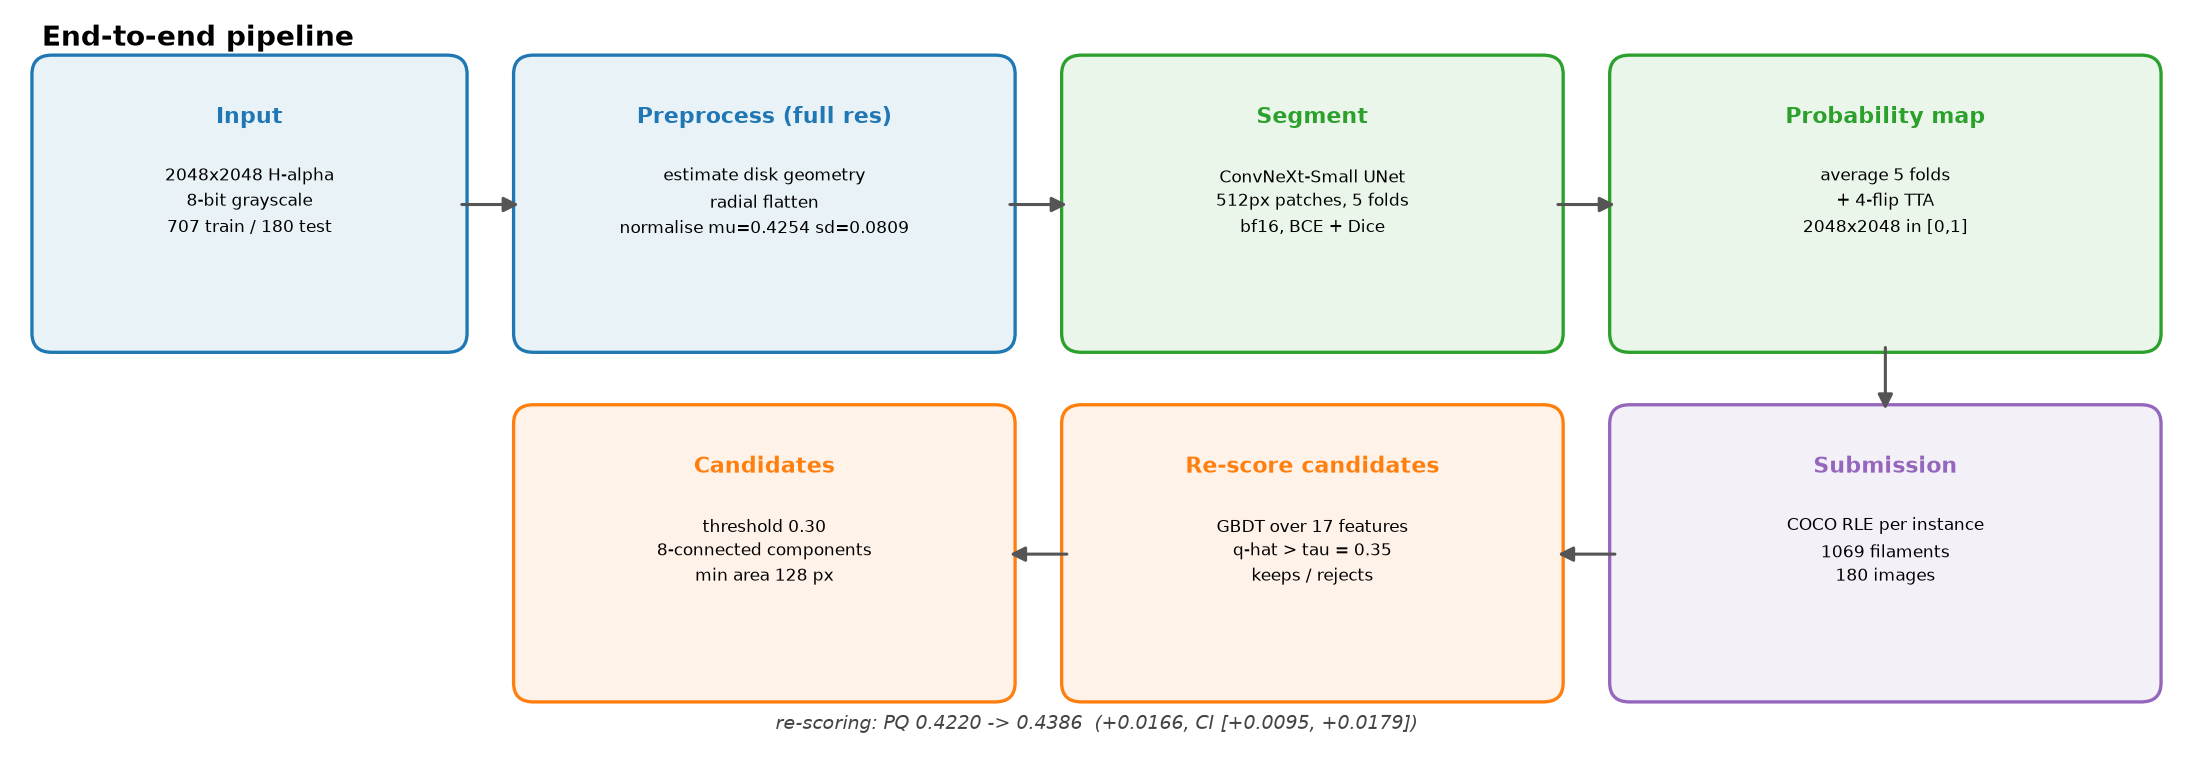
\includegraphics[width=0.95\textwidth]{figures/pipeline.png}
\caption{End-to-end data pipeline. Preprocessing runs at full resolution because radial flattening estimates its background profile from annuli spanning the whole disk. The five-fold ensemble is averaged in probability space before thresholding, and connected components of the averaged map are re-ranked by a gradient-boosted model.}
\label{fig:pipeline}
\end{figure*}

\begin{figure*}[t]
\centering
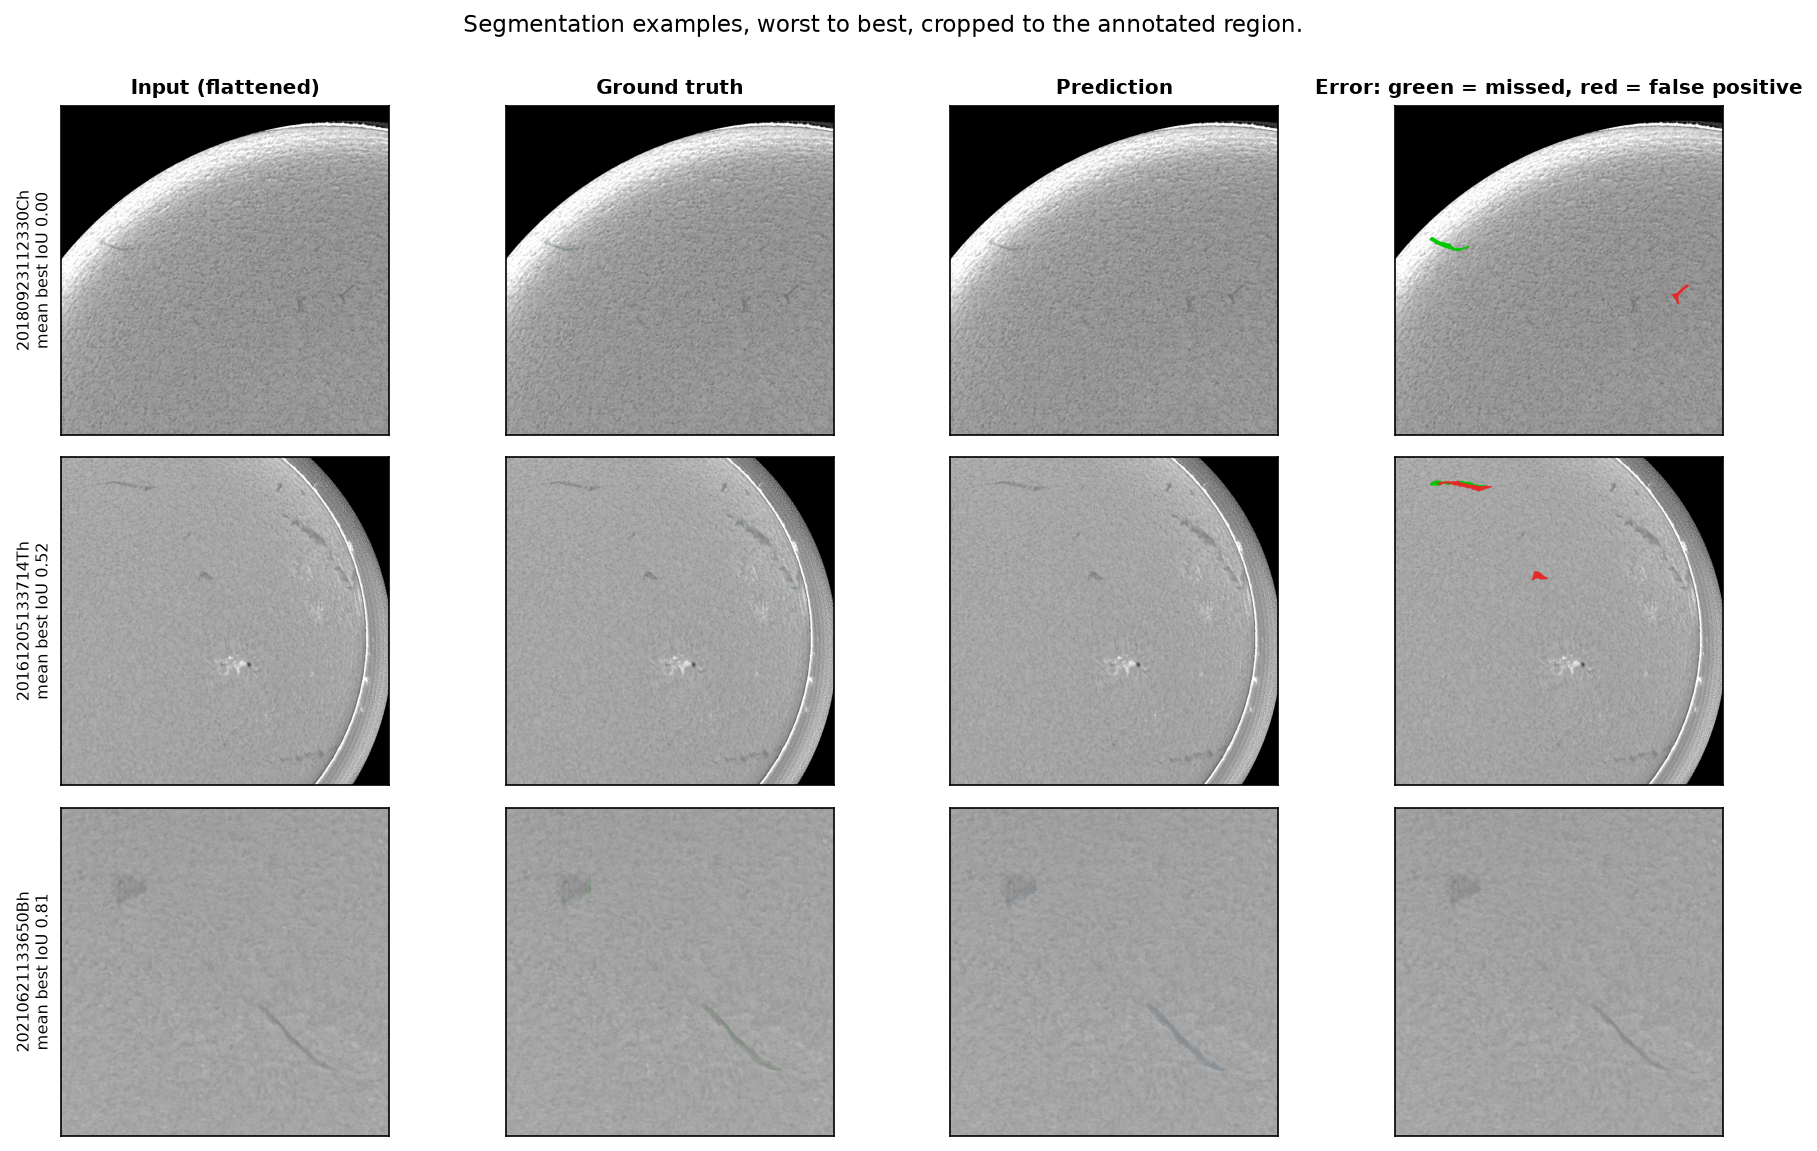
\includegraphics[width=0.95\textwidth]{figures/segmentation_examples.png}
\caption{Segmentation examples, ordered worst to best and cropped to the annotated region (a filament occupies $\sim0.3\%$ of a full-disk image, so a full view shows nothing). Green marks a missed ground-truth filament, red a false positive. The top row is a complete failure; the bottom row is a near-perfect match. The failure mode is consistently a filament that is faint or near the limb and is not detected at all, not one that is detected with a poor boundary.}
\label{fig:examples}
\end{figure*}


% ==================================== %
%              EVALUATION              %
% ==================================== %
\section{Evaluation}\label{sec:evaluation}

\subsection{Overall results}
    Table~\ref{tab:results} reports the four configurations we evaluated. The segmentation baseline reaches PQ $0.4220$; candidate re-scoring raises it to $0.4386$, a paired gain of $+0.0166$ with a $95\%$ bootstrap CI of $[+0.0095, +0.0179]$ over 2{,}000 resamples of the 707 files. The public leaderboard score is $0.38$.

    The row reported is the configuration we actually submitted: the GBDT scorer alone at an absolute $\tau=0.35$. A rank-average blend of the GBDT and a small CNN scored marginally higher on OOF ($0.4406$), but its threshold is a \emph{quantile} of the candidate score distribution, and that distribution shifts on test---$11.7\%$ of test files are from 2021--22 against $5.7\%$ of training files. An absolute threshold on a calibrated score transfers; a rank threshold does not. The blend's $+0.0020$ is also well inside the CI width, so we did not spend a submission on it.

\begin{table}[t]
\centering
\caption{Pooled out-of-fold results. SQ and RQ are the factors of PQ. The last two rows are interventions that were rejected.}
\label{tab:results}
\small
\begin{tabular}{@{}lccc@{}}
\toprule
Configuration & PQ & SQ & RQ \\
\midrule
Segmentation only        & 0.4220 & 0.6765 & 0.6238 \\
+ candidate re-scoring   & \textbf{0.4386} & 0.6786 & 0.6464 \\
\midrule
+ GONG label transfer    & 0.4045 & 0.6667 & 0.6095 \\
+ PVTv2-B2 ensemble      & 0.4098 & 0.6719 & 0.6099 \\
\bottomrule
\end{tabular}
\end{table}

\subsection{SQ does not move}
    The most informative column of Table~\ref{tab:results} is SQ. Across four architectures---resnet34, DeepCrack with a decoder, ConvNeXt-Small, and PVTv2-B2 \cite{pvt}---SQ stays within $0.667$--$0.679$. Re-scoring improves RQ by $+0.023$ and SQ by only $+0.002$.

    This is a strong constraint. If boundary precision were the bottleneck, a transformer with global receptive field should have moved SQ. It did not. The network is already delineating filaments about as well as this supervision allows, and the remaining error lies elsewhere.

\subsection{The error is missed instances}
    To locate it, we measured the full IoU and Dice distributions over all 707 out-of-fold files with the shipped post-processing. Table~\ref{tab:dist} reports three populations, because a single histogram is ambiguous: quoting only matched pairs flatters the system by hiding misses, while quoting only per-object values hides that boundaries are good when the instance is found.

\begin{table}[t]
\centering
\caption{IoU and Dice over three populations. ``Per ground-truth'' scores missed instances as 0; ``per prediction'' scores false positives as 0.}
\label{tab:dist}
\small
\begin{tabular}{@{}lcccc@{}}
\toprule
Population & $n$ & IoU & Dice & Dice $\geq 0.75$ \\
\midrule
Matched pairs      & 5{,}259 & 0.677 & 0.804 & 77.5\% \\
Per ground-truth   & 8{,}199 & 0.501 & 0.614 & 49.7\% \\
Per prediction     & 8{,}662 & 0.481 & 0.591 & 47.0\% \\
\bottomrule
\end{tabular}
\end{table}

    The gap between the first two rows is the finding. When an instance is matched, Dice averages $0.804$ and $77.5\%$ of matches exceed $0.75$: the boundaries are good. Across all ground-truth instances the mean falls to $0.614$, because $16.7\%$ of filaments score below $0.10$---they were missed entirely. Fig.~\ref{fig:dice} shows the same thing as a distribution. Recall is $0.641$ and precision $0.607$; both are mediocre, but a missed filament is unrecoverable whereas a false positive at least had a chance of being right.

\begin{figure*}[t]
\centering
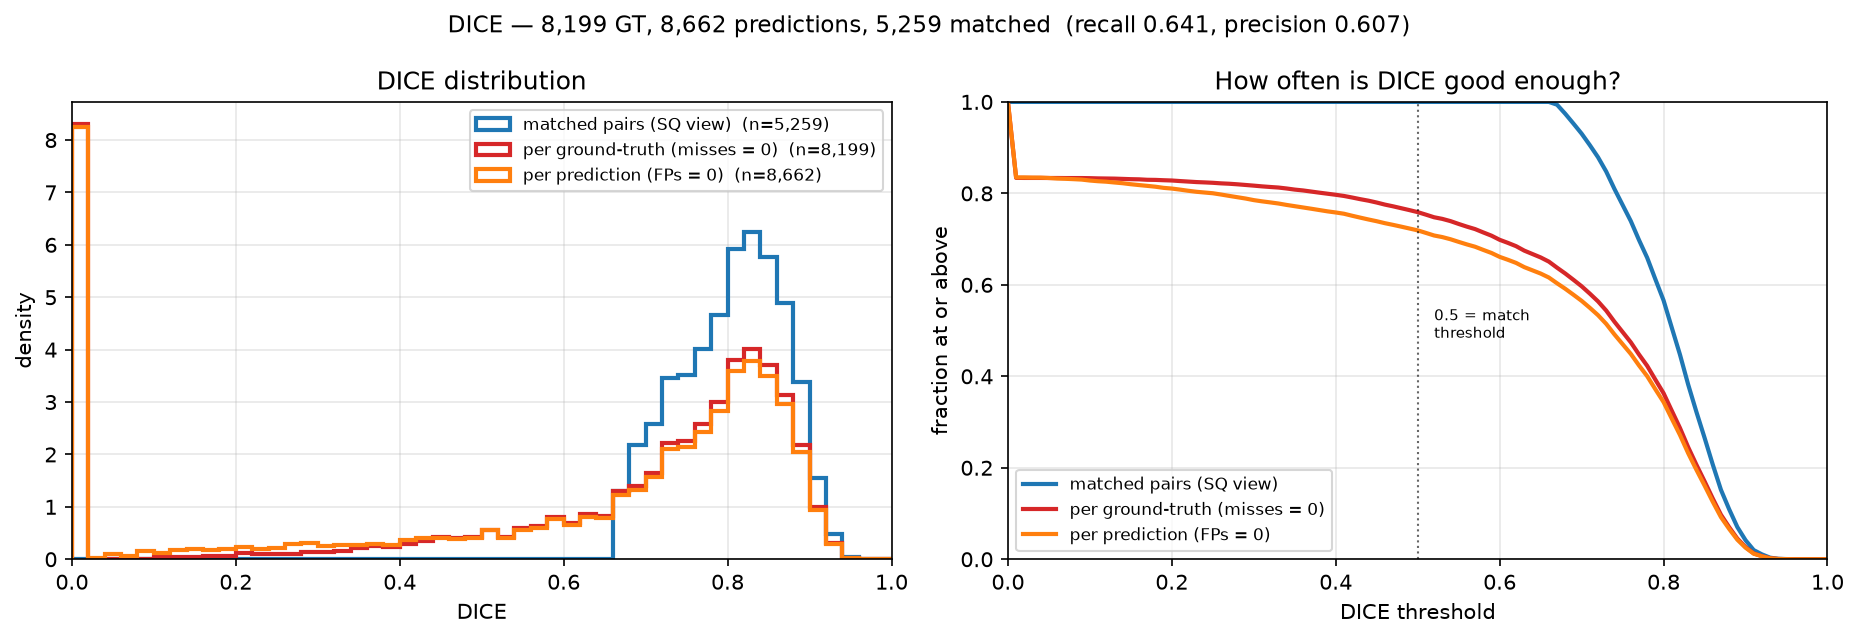
\includegraphics[width=0.86\textwidth]{figures/dice_distribution.png}
\caption{Dice over three populations. The matched-pair curve (blue) sits well above the per-object curves (red, orange); the mass at zero in the latter is missed filaments and false positives. Left: density. Right: the fraction of each population reaching at least a given Dice, which is the form in which the $16.7\%$ miss rate is directly readable.}
\label{fig:dice}
\end{figure*}

\subsection{No fragmentation, no merging}
    PQ's denominator charges $\tfrac12|\mathrm{FP}| + \tfrac12|\mathrm{FN}|$, so splitting one filament into three costs almost as much as missing it. This motivated a fragment-merging stage in our original plan, based on an early analysis that attributed $58.5\%$ of false positives to fragments.

    That analysis was wrong. Measuring the false-positive anatomy over all 707 files gives $47.3\%$ background, $51.0\%$ unmatched ground truth, and \emph{$1.8\%$} fragments. The oracle gain from removing every fragment is $+0.0015$ PQ. Table~\ref{tab:rel} shows why: at the metric's own threshold of $\mathrm{IoU}>0.5$ there is no fragmentation and no merging at all. Multi-relations appear only at loose overlaps, where a prediction grazes a neighbouring filament without competing for the match.

\begin{table}[t]
\centering
\caption{Instance relations. At the matching threshold of 0.5 the multi-relations vanish entirely.}
\label{tab:rel}
\small
\begin{tabular}{@{}lcc@{}}
\toprule
Relation & IoU $> 0.1$ & IoU $> 0.5$ \\
\midrule
One GT split by $k>1$ predictions & 4.8\% & 0.0\% \\
One prediction merging $k>1$ GT   & 1.8\% & 0.0\% \\
\bottomrule
\end{tabular}
\end{table}

\subsection{Two interventions that failed}
    \textbf{More data, from the wrong observation.} The competition images are GONG H-$\alpha$ frames \cite{gong}, so annotations can in principle be transferred from nearby frames in the public archive. We verified that the competition images \emph{are} the GONG \texttt{hag} JPEGs (correlation $0.997$, median absolute difference 1 count, best alignment shift $(0,0)$), which made transfer feasible without radiometric correction. Transferring labels from nearby frames produced $3.1\times$ the training data and a PQ change of $-0.0150$. The per-year breakdown explains it: gains appeared exactly where the extra frames were concentrated (2021--22, $+0.0109$), and losses appeared in years where transferred labels came from a different observation (2011: $-0.0475$; 2016: $-0.0426$; 2017: $-0.0389$). SQ fell from $0.6750$ to $0.6667$. Solar filaments evolve over hours; a polygon drawn on a frame six hours earlier describes a different object, and training on it teaches the model to be imprecise about boundaries.

    \textbf{Architectural diversity without error diversity.} Ensembles help when members make \emph{uncorrelated} errors. Our five ConvNeXt folds share an architecture, a preprocessing pipeline and a loss, so averaging them mostly reduces variance. A pyramid vision transformer (PVTv2-B2) was expected to fail differently: self-attention gives every output position a path to every input position, so a filament is seen as a whole shape rather than through stacked local receptive fields. PVTv2 scored $0.3906$ solo against ConvNeXt's $0.4177$, which is expected for a diversity member. But averaging the two gave $-0.0113$ (CI $[-0.0239, +0.0001]$). The mechanism is one number: the two models' predictions correlate at $\mathbf{0.913}$. Two predictors that agree on $91\%$ of pixels cannot cancel each other's mistakes; the average lands between them and below the better one.

\subsection{Strengths, weaknesses, and next steps}
    The system's strength is that it is well calibrated about \emph{what it has found}: matched instances reach Dice $0.804$, and the re-scoring stage removes false positives without deleting true filaments. Its weakness is recall. Scoring every candidate with its true label gives an oracle ceiling of PQ $0.5028$, i.e.\ $+0.0808$ above the segmentation baseline; the learned scorer captures $+0.0166$ of that ($21\%$), leaving $+0.0642$ unclaimed.

    This is the largest known opportunity, and it is a ranking problem rather than a segmentation problem. Since the error is dominated by missed instances, and those instances are largely \emph{present as candidates} and being discarded, the productive direction is a scorer optimised for recall against PQ's instance-count objective rather than for average precision. A scorer trained to maximise average precision will happily discard low-confidence candidates that are nonetheless true positives, because they contribute little to the ranking metric; PQ does not care about ranking, only about the count of matched instances. That objective mismatch is a plausible explanation for capturing only $23\%$ of the oracle gap.

    A limitation worth stating: all local numbers are pooled out-of-fold on 707 training images, and the public leaderboard is a two-decimal readout on roughly half the test set. The local-to-public gap is $0.0586$ and is \emph{not} constant across component types, so it is not a fixed offset to subtract. The test set is also shifted---$11.7\%$ of test files are from 2021--22 against $5.7\%$ of training files---and since label transfer showed sensitivity to observation epoch, this is a plausible contributor we have not isolated.



% ==================================== %
%            ACKNOWLEDGMENT            %
% ==================================== %
\section{Acknowledgment}\label{sec:acknowledgment}
    % Do not change
    The organization of the Filament Segmentation Challenge 2026 is partially supported by the U.S. National Science Foundation (NSF) under Grant No. 2209912 and 2433781, directorate for Computer and Information Science and Engineering (CSE), and Office of Advanced Cyberinfrastructure (OAC), and Grant No. 2511630, AST Division Of Astronomical Sciences and MPS Directorate for Mathematical and Physical Sciences.

    The Filament Segmentation Challenge 2026 is sponsored by the U.S. National Science Foundation (NSF) National Solar Observatory (NSO). 

    This work utilizes GONG data obtained by the NSO Integrated Synoptic Program, managed by the National Solar Observatory, which is operated by the Association of Universities for Research in Astronomy (AURA), Inc. under a cooperative agreement with the National Science Foundation and with contribution from the National Oceanic and Atmospheric Administration. The GONG network of instruments is hosted by the Big Bear Solar Observatory, High Altitude Observatory, Learmonth Solar Observatory, Udaipur Solar Observatory, Instituto de Astrofísica de Canarias, and Cerro Tololo Interamerican Observatory.

\bibliographystyle{ACM-Reference-Format}
\bibliography{main}

\end{document}
